\documentclass[border=10pt]{standalone}

% Pacchetti necessari
\usepackage[T1]{fontenc}
\usepackage{amsmath}
\usepackage{amssymb}
\usepackage{graphicx}
\usepackage{caption}
\usepackage{subcaption}
\usepackage{tikz}
\usepackage{pgfplots}
\usepackage{booktabs}
\usepackage{multirow}
\usepackage{fontspec}
\usepackage{pgfplotstable}
\usepackage{tikz-3dplot}

\captionsetup{font=small, labelfont=bf, labelsep=period}
\pgfplotsset{compat=1.17}
\usetikzlibrary{patterns,arrows.meta,shapes,positioning,calc,backgrounds,fit,decorations.pathreplacing,pgfplots.polar}

\setmainfont{Arial} % Richiede XeLaTeX o LuaLaTeX per la compilazione

\definecolor{gdoblu}{RGB}{52, 152, 219}
\definecolor{gdoverde}{RGB}{46, 204, 113}

% --- COMANDI PERSONALIZZATI PER LE METRICHE ---
\newcommand{\metric}[1]{{\footnotesize #1}}
\newcommand{\metricvalue}[1]{{\footnotesize\bfseries\color{green!70!black} #1}}
\newcommand{\metricnote}[1]{{\scriptsize\color{gray} #1}}

\begin{document}

\centering
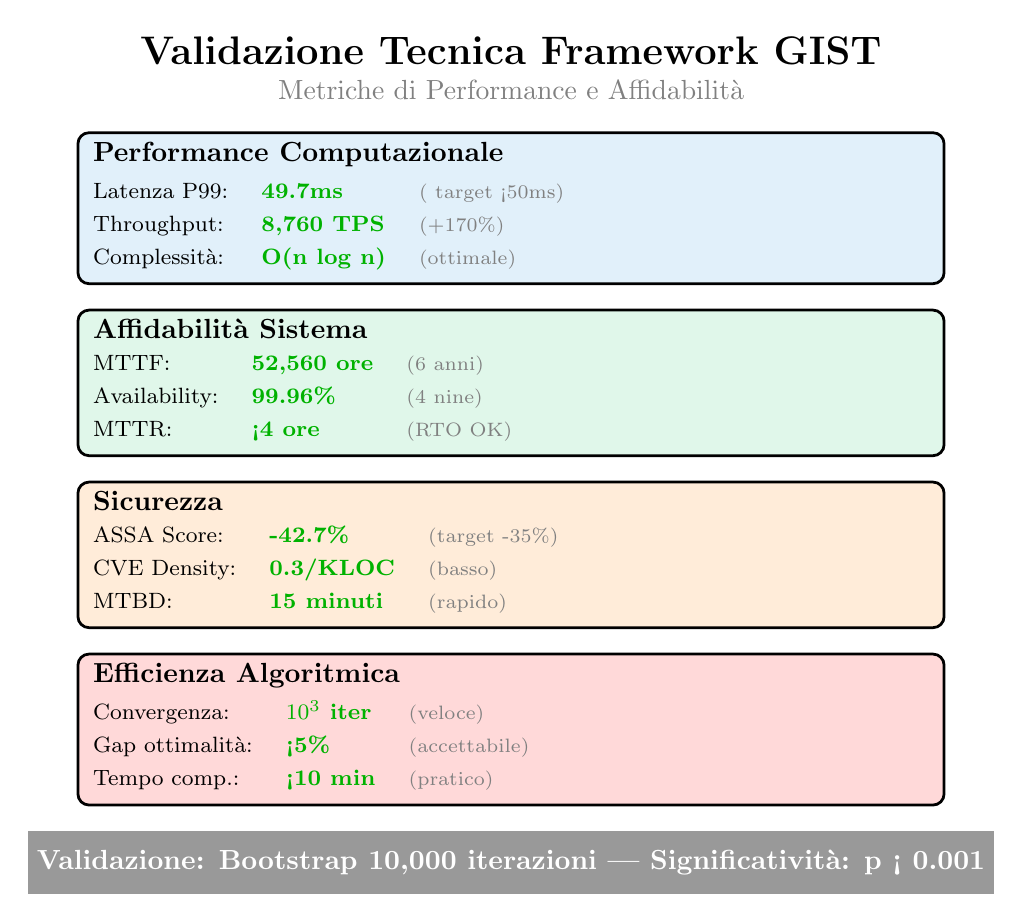
\begin{tikzpicture}[
    % Gli stili per le metriche sono stati rimossi da qui
    box/.style={rectangle, rounded corners, draw=black, line width=1pt, minimum width=11cm}
]

% Titolo
\node[font=\Large\bfseries] at (0,0) {Validazione Tecnica Framework GIST};
\node[font=\normalsize, text=gray] at (0,-0.5) {Metriche di Performance e Affidabilità};

% Performance Computazionale
\node[box, fill=gdoblu!15, align=left] (perf) at (0,-2) {
    \begin{minipage}{10.5cm}
    \textbf{Performance Computazionale}\\[2pt]
    \begin{tabular}{@{}lll@{}}
    \metric{Latenza P99:} & \metricvalue{49.7ms} & \metricnote{( target <50ms)} \\
    \metric{Throughput:} & \metricvalue{8,760 TPS} & \metricnote{(+170\%)} \\
    \metric{Complessità:} & \metricvalue{O(n log n)} & \metricnote{(ottimale)}
    \end{tabular}
    \end{minipage}
};

% Affidabilità Sistema
\node[box, fill=gdoverde!15, align=left, below=0.3cm of perf] (reliability) {
    \begin{minipage}{10.5cm}
    \textbf{Affidabilità Sistema}\\[2pt]
    \begin{tabular}{@{}lll@{}}
    \metric{MTTF:} & \metricvalue{52,560 ore} & \metricnote{(6 anni)} \\
    \metric{Availability:} & \metricvalue{99.96\%} & \metricnote{(4 nine)} \\
    \metric{MTTR:} & \metricvalue{<4 ore} & \metricnote{(RTO OK)}
    \end{tabular}
    \end{minipage}
};

% Sicurezza
\node[box, fill=orange!15, align=left, below=0.3cm of reliability] (security) {
    \begin{minipage}{10.5cm}
    \textbf{Sicurezza}\\[2pt]
    \begin{tabular}{@{}lll@{}}
    \metric{ASSA Score:} & \metricvalue{-42.7\%} & \metricnote{(target -35\%)} \\
    \metric{CVE Density:} & \metricvalue{0.3/KLOC} & \metricnote{(basso)} \\
    \metric{MTBD:} & \metricvalue{15 minuti} & \metricnote{(rapido)}
    \end{tabular}
    \end{minipage}
};

% Efficienza Algoritmica
\node[box, fill=red!15, align=left, below=0.3cm of security] (efficiency) {
    \begin{minipage}{10.5cm}
    \textbf{Efficienza Algoritmica}\\[2pt]
    \begin{tabular}{@{}lll@{}}
    \metric{Convergenza:} & \metricvalue{$10^3$ iter} & \metricnote{(veloce)} \\
    \metric{Gap ottimalità:} & \metricvalue{<5\%} & \metricnote{(accettabile)} \\
    \metric{Tempo comp.:} & \metricvalue{<10 min} & \metricnote{(pratico)}
    \end{tabular}
    \end{minipage}
};

% Footer
\node[rectangle, fill=gray!80, text=white, minimum width=11cm, minimum height=0.8cm, below=0.3cm of efficiency] {
    \textbf{Validazione: Bootstrap 10,000 iterazioni | Significatività: p < 0.001}
};

\end{tikzpicture}

\end{document}